\documentclass[letter,12pt]{article}
\usepackage[paperheight=27.94cm,paperwidth=21.59cm,bindingoffset=0in,left=3cm,right=2.0cm, top=3.5cm,bottom=2.5cm, headheight=200pt, headsep=1.0\baselineskip]{geometry}
\usepackage{graphicx,lastpage}
\usepackage{upgreek}
\usepackage{censor}
\usepackage[spanish,es-tabla]{babel}
\usepackage{pdfpages}
\usepackage{tabularx}
\usepackage{graphicx}
\usepackage{adjustbox}
\usepackage{xcolor}
\usepackage{colortbl}
\usepackage{rotating}
\usepackage{multirow}
\usepackage[utf8]{inputenc}
\usepackage{float}
\usepackage{hyperref}
\usepackage{subcaption}
\usepackage{booktabs}
\newcolumntype{P}[1]{>{\raggedright\arraybackslash}p{#1}}
\setlength{\parindent}{0pt}

\renewcommand{\tablename}{Tabla}
\usepackage{fancyhdr}
\pagestyle{fancy}

\fancyhead[L]{}
%
\begin{document}
%
   \title{\Huge{Informe Laboratorio 2}}

   \author{\textbf{Sección x} \\  \\Alumno x \\ e-mail: alumno.contacto@mail.udp.cl}
          
   \date{Septiembre de 2024}

   \maketitle
   
   \tableofcontents
 
  \newpage
  

\section{Descripción de actividades}
Utilizando la aplicación web vulnerable DVWA

(Damn Vulnerable Web App - \href{https://github.com/digininja/DVWA}{https://github.com/digininja/DVWA} (Enlaces a un sitio externo.)) realice las siguientes actividades:


\begin{itemize}
    \item Despliegue la aplicación en su equipo utilizando docker. Detalle el procedimiento y explique los parámetros que utilizó.
    \item Utilice Burpsuite (https://portswigger.net/burp/communitydownload (Enlaces a un sitio externo.)) para realizar un ataque de fuerza bruta contra formulario ubicado en vulnerabilities/brute. Explique el proceso y obtenga al menos 2 pares de usuario/contraseña válidos. Muestre las diferencias observadas en burpsuite.
    \item Utilice la herramienta cURL, a partir del código obtenido de inspect elements de su navegador, para realizar un acceso válido y uno inválido al formulario ubicado en vulnerabilities/brute. Indique 4 diferencias entre la página que retorna el acceso válido y la página que retorna un acceso inválido.
    \item Utilice la herramienta Hydra para realizar un ataque de fuerza bruta contra formulario ubicado en vulnerabilities/brute. Explique el proceso y obtenga al menos 2 pares de usuario/contraseña válidos.
    \item Compare los paquetes generados por hydra, burpsuite y cURL. ¿Qué diferencias encontró? ¿Hay forma de detectar a qué herramienta corresponde cada paquete?

    \item Desarrolle un script en Python para realizar un ataque de fuerza bruta:

    \begin{itemize}
        \item Utilice la librería requests para interactuar con el formulario ubicado en vulnerabilities/brute y desarrollar su propio script de fuerza bruta en Python.
        El script debe realizar intentos de inicio de sesión probando una lista de combinaciones de usuario/contraseña.

        \item  Identifique y explique la cabecera HTTP que empleará para realizar el ataque de fuerza bruta.

        \item  Muestre el código y los resultados obtenidos (al menos 2 combinaciones válidas de usuario/contraseña).

        \item Compare el rendimiento de este script en Python con las herramientas Hydra, Burpsuite, y cURL en términos de velocidad y detección.
    \end{itemize}

    \item  Investigue y describa 4 métodos comunes para prevenir o mitigar ataques de fuerza bruta en aplicaciones web:

    \begin{itemize}
        \item Para cada método, explique su funcionamiento, destacando en qué escenarios es más eficaz.

    \end{itemize}


    
\end{itemize}

%DE AQUI HAY QUE COMENZAR A ESCRIBIR%


\section{Desarrollo de actividades según criterio de rúbrica}

\subsection{Levantamiento de docker para correr DVWA (dvwa)}

Para el despliegue de la aplicación se clonó el repositorio oficial de DVWA desde
\url{https://github.com/digininja/DVWA}, tal como se ilustra en la Figura~\ref{fig:clonar}.

\begin{figure}[H]
    \centering
    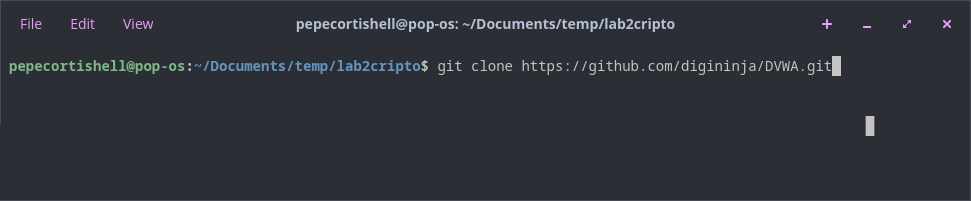
\includegraphics[width=0.85\textwidth]{img/01-1-clonarRepositorio.png}
    \caption{Clonación del repositorio DVWA.}
    \label{fig:clonar}
\end{figure}

Posteriormente, desde el interior del directorio clonado, se inició el contenedor Docker mediante el comando
\texttt{sudo docker compose up -d} (Figura~\ref{fig:contenedor}).

\begin{figure}[H]
    \centering
    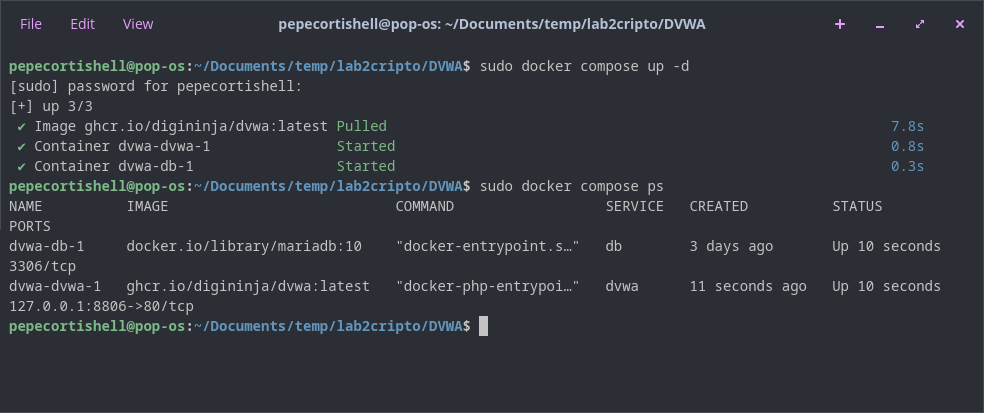
\includegraphics[width=0.85\textwidth]{img/01-2-levantarContenedor.png}
    \caption{Levantamiento del contenedor Docker con DVWA.}
    \label{fig:contenedor}
\end{figure}

Una vez levantado el contenedor, se verificó su correcto funcionamiento accediendo a
\url{http://localhost:8806/login.php} e iniciando sesión con las credenciales
\texttt{admin~/ password} (Figura~\ref{fig:login}).

\begin{figure}[H]
    \centering
    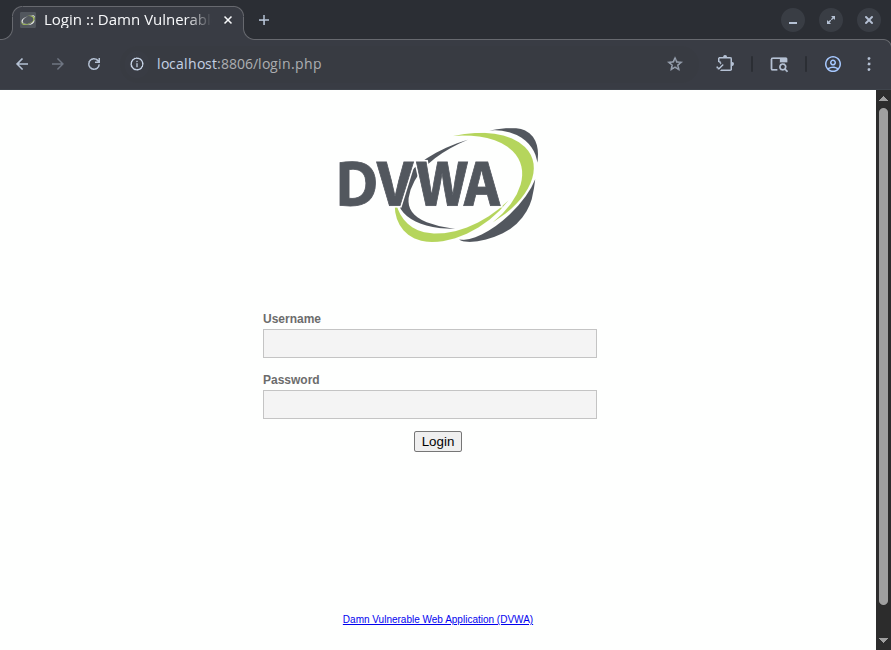
\includegraphics[width=0.85\textwidth]{img/01-3-login.png}
    \caption{Inicio de sesión en DVWA.}
    \label{fig:login}
\end{figure}

A continuación, se inicializó la base de datos de la aplicación desde la página de configuración
\url{http://localhost:8806/setup.php} (Figura~\ref{fig:bbdd}).

\begin{figure}[H]
    \centering
    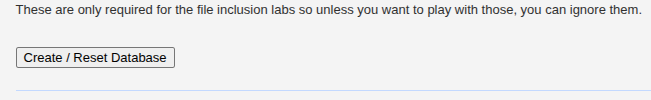
\includegraphics[width=0.85\textwidth]{img/01-3-crearBBDD.png}
    \caption{Creación de la base de datos desde el panel de configuración.}
    \label{fig:bbdd}
\end{figure}

Finalmente, se estableció el nivel de seguridad en \textit{Low} desde
\url{http://localhost:8806/security.php}, reduciendo las protecciones de la aplicación
para facilitar la ejecución de los ejercicios propuestos (Figura~\ref{fig:security}).

\begin{figure}[H]
    \centering
    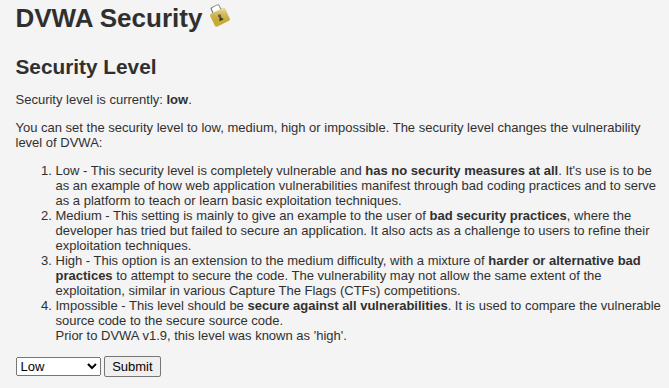
\includegraphics[width=0.85\textwidth]{img/01-4-securityLow.png}
    \caption{Configuración del nivel de seguridad en \textit{Low}.}
    \label{fig:security}
\end{figure}

\subsection{Redirección de puertos en docker (dvwa)}

Para acceder a la aplicación desde el equipo anfitrión, se configuró un mapeo de puertos
en el archivo \texttt{compose.yml} del repositorio clonado. Se asignó el puerto 8806 del
host al puerto 80 del contenedor mediante la directiva \texttt{ports: "8806:80"},
de modo que cualquier petición dirigida a \url{http://localhost:8806} es reenviada
internamente al puerto 80 donde la aplicación DVWA se encuentra en ejecución
(Figura~\ref{fig:puertos}).

\begin{figure}[H]
    \centering
    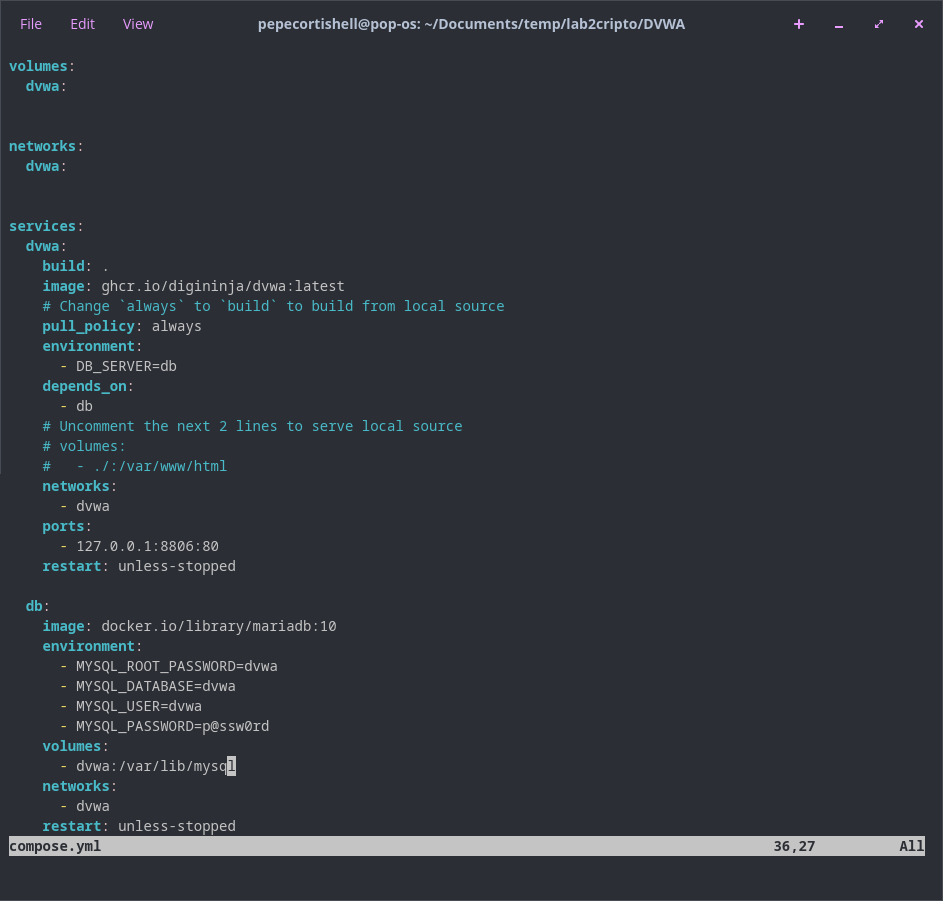
\includegraphics[width=0.85\textwidth]{img/02-1-redireccionPuertos.png}
    \caption{Configuración del mapeo de puertos en \texttt{compose.yml}.}
    \label{fig:puertos}
\end{figure}

\subsection{Obtención de consulta a replicar (burp)}

Se accedió a Burp Suite y se habilitó la intercepción de tráfico HTTP. A continuación, se
completó el formulario de autenticación ubicado en
\url{http://localhost:8806/vulnerabilities/brute/} con credenciales arbitrarias y se
ejecutó el envío. La herramienta interceptó la solicitud resultante, correspondiente a un
request \texttt{GET} con los parámetros \texttt{username}, \texttt{password} y
\texttt{Login} adjuntos en la URL. Dicha solicitud fue derivada al módulo
\textit{Intruder} para su posterior análisis y configuración del ataque
(Figura~\ref{fig:requestGET}).

\begin{figure}[H]
    \centering
    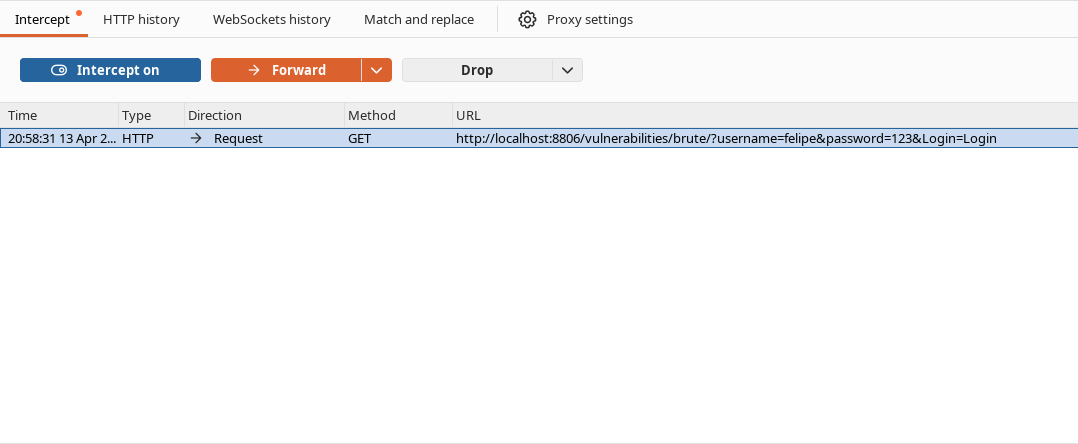
\includegraphics[width=0.85\textwidth]{img/03-1-requestGET.png}
    \caption{Request GET interceptado en Burp Suite correspondiente al formulario de \textit{vulnerabilities/brute}.}
    \label{fig:requestGET}
\end{figure}

\subsection{Identificación de campos a modificar (burp)}

Dentro del módulo \textit{Intruder} de Burp Suite, se identificaron los query parameters
\texttt{username} y \texttt{password} del request GET como las posiciones de payload a
iterar. Estos parámetros se transmiten en la URL bajo la forma
\texttt{?username=\$valor\$\&password=\$valor\$\&Login=Login}. Se seleccionó el
modo de ataque \textit{Cluster Bomb}, el cual permite combinar de forma independiente
dos listas de valores, generando todas las combinaciones posibles entre los usuarios y las
contraseñas del diccionario (Figura~\ref{fig:intruder}).

\begin{figure}[H]
    \centering
    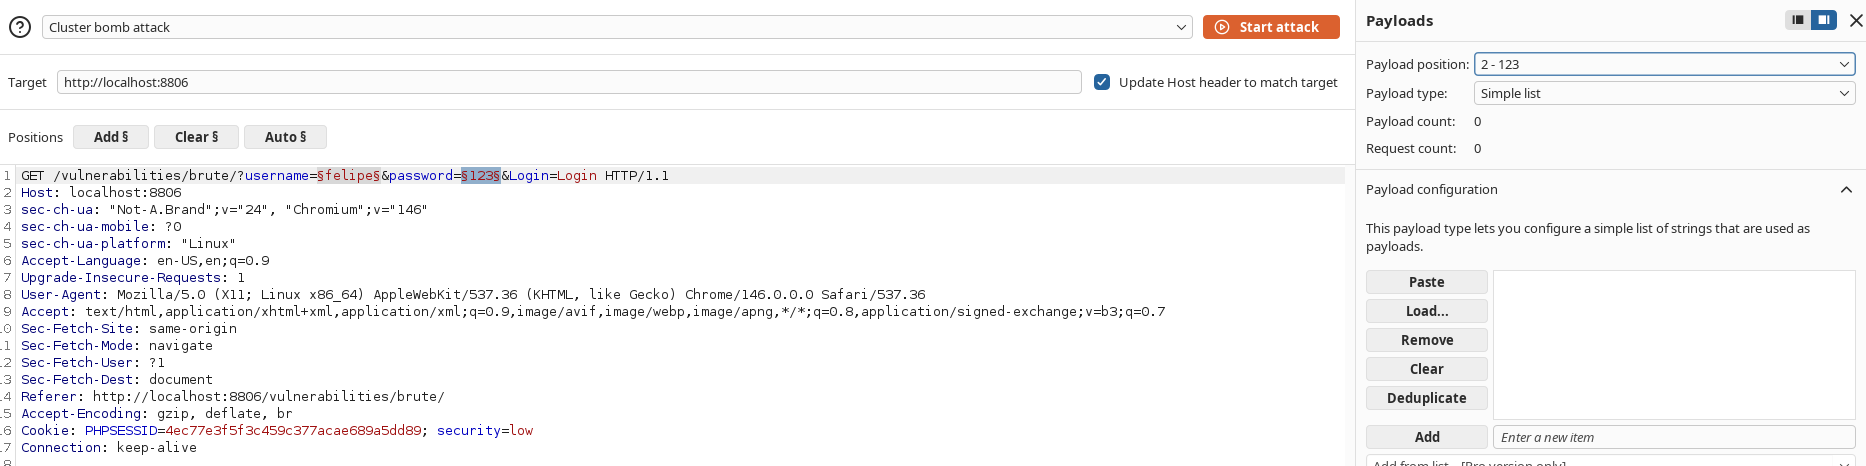
\includegraphics[width=0.85\textwidth]{img/04-1-intruder.png}
    \caption{Configuración del ataque en Burp Suite \textit{Intruder} con los query parameters \texttt{username} y \texttt{password} como posiciones de payload.}
    \label{fig:intruder}
\end{figure}

\subsection{Obtenci\'{o}n de diccionarios para el ataque (burp)}

Se elaboraron dos diccionarios de tamaño reducido: uno de usuarios y uno de contraseñas.
Ambos fueron construidos a partir de ejemplos extraídos del repositorio
\textit{SecLists} disponible en \url{https://github.com/danielmiessler/SecLists},
complementados con valores que se conocían de antemano como válidos para la aplicación.
El uso de diccionarios completos del repositorio fue descartado, dado que la combinación
de 40.000 usuarios con 40.000 contraseñas genera $1.6 \times 10^{9}$ combinaciones,
lo que haría inviable el ataque en el tiempo disponible. En su lugar, se utilizaron
diccionarios de aproximadamente 20 entradas cada uno
(Figura~\ref{fig:diccionarios}).

\begin{figure}[H]
    \centering
    \begin{minipage}[t]{0.48\textwidth}
        \centering
        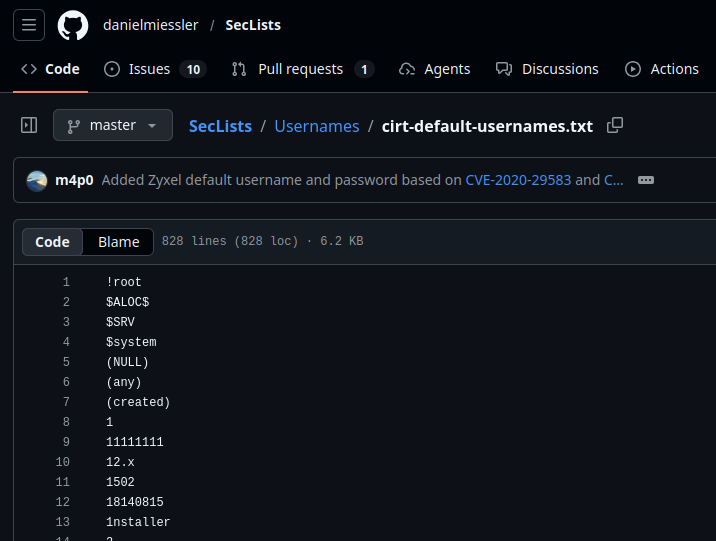
\includegraphics[width=\textwidth]{img/05-1-dicUsername.png}
        \subcaption{Diccionario de usuarios.}
    \end{minipage}
    \hfill
    \begin{minipage}[t]{0.48\textwidth}
        \centering
        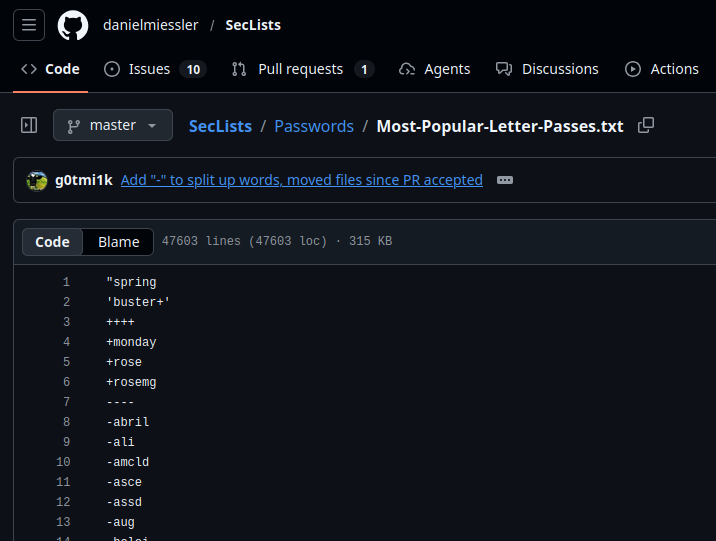
\includegraphics[width=\textwidth]{img/05-2-dicPassword.png}
        \subcaption{Diccionario de contraseñas.}
    \end{minipage}
    \caption{Diccionarios utilizados para el ataque, construidos a partir de ejemplos de SecLists.}
    \label{fig:diccionarios}
\end{figure}

\subsection{Obtenci\'{o}n de al menos 2 pares (burp)}

En la sección de configuración de payloads del \textit{Intruder}, se importaron los
diccionarios \texttt{u.txt} y \texttt{p.txt} como \textit{Simple List} para los
query parameters \texttt{username} y \texttt{password}, respectivamente
(Figura~\ref{fig:payloads}).

\begin{figure}[H]
    \centering
    \begin{minipage}[t]{0.48\textwidth}
        \centering
        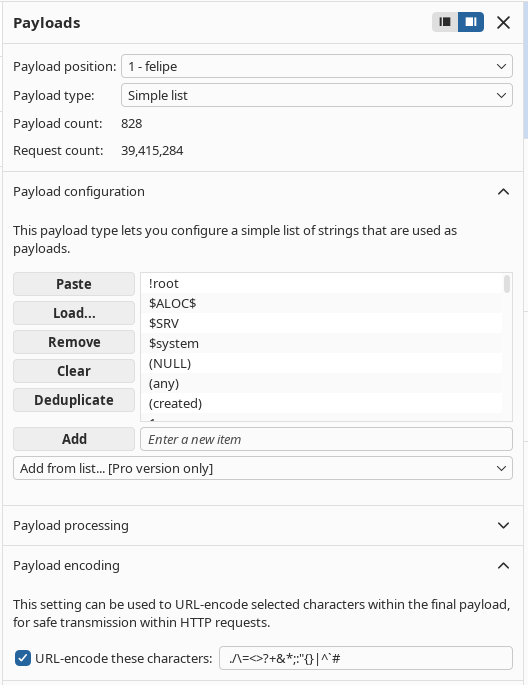
\includegraphics[width=\textwidth]{img/06-1-usernamePayload.png}
        \subcaption{Payload para \texttt{username}.}
    \end{minipage}
    \hfill
    \begin{minipage}[t]{0.48\textwidth}
        \centering
        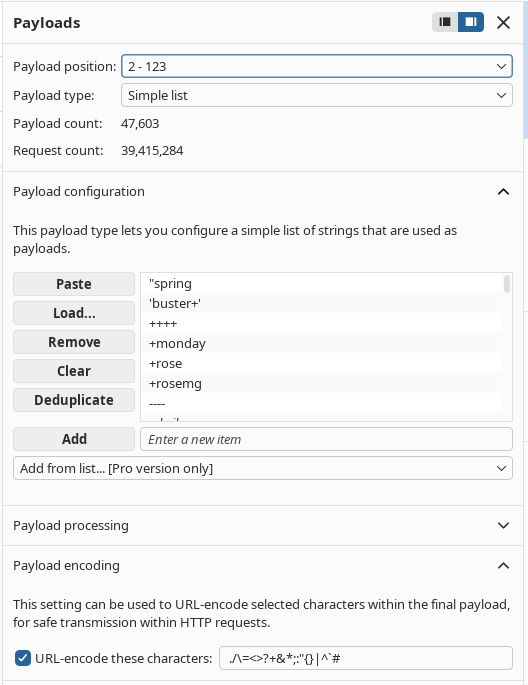
\includegraphics[width=\textwidth]{img/06-2-passwordPayload.png}
        \subcaption{Payload para \texttt{password}.}
    \end{minipage}
    \caption{Configuración de los payloads en Burp Suite \textit{Intruder}.}
    \label{fig:payloads}
\end{figure}

Para identificar los intentos fallidos, se configuró un filtro \textit{Grep Match} con
el texto \texttt{Username and/or password incorrect}. Este mensaje aparece en el cuerpo
de la respuesta HTTP cuando las credenciales enviadas no son válidas, permitiendo así
distinguir los intentos exitosos de los fallidos (Figura~\ref{fig:grepMatch}).

\begin{figure}[H]
    \centering
    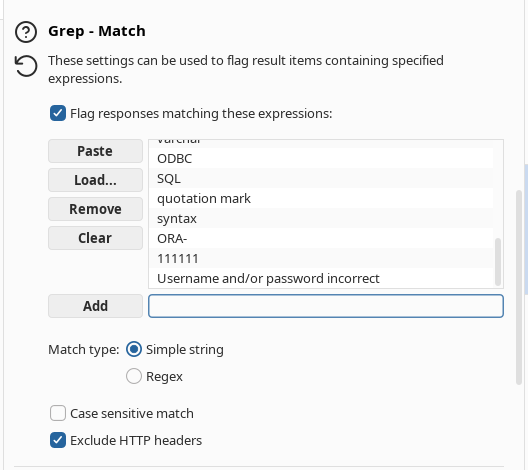
\includegraphics[width=0.85\textwidth]{img/06-3-GrepMatch.png}
    \caption{Configuración del filtro \textit{Grep Match} en Burp Suite \textit{Intruder}.}
    \label{fig:grepMatch}
\end{figure}

Una vez ejecutado el ataque sobre las 280 combinaciones posibles, se filtraron los
resultados por el \textit{Grep Match} definido y se identificaron los siguientes pares
de credenciales válidos: \texttt{pablo / letmein} y \texttt{gordonb / abc123}
(Figura~\ref{fig:paresValidos}).

\begin{figure}[H]
    \centering
    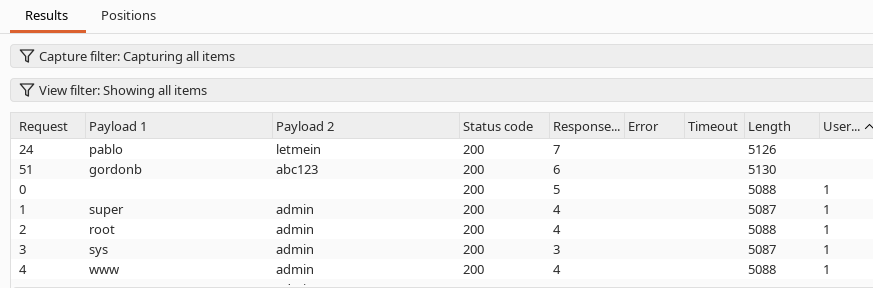
\includegraphics[width=0.85\textwidth]{img/06-4-paresValidos.png}
    \caption{Resultados del ataque en Burp Suite: pares de credenciales válidos obtenidos.}
    \label{fig:paresValidos}
\end{figure}

A modo de verificación, se utilizaron las credenciales \texttt{pablo / letmein} en el
formulario de \url{http://localhost:8806/vulnerabilities/brute/}, obteniendo como
respuesta el mensaje \textit{``Welcome to the password protected area pablo''},
confirmando la validez del par obtenido (Figura~\ref{fig:loginValido}).

\begin{figure}[H]
    \centering
    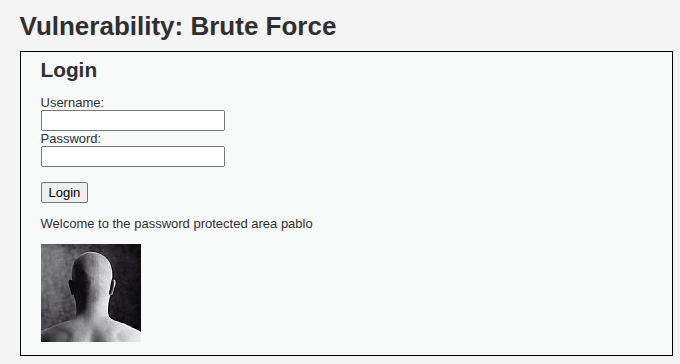
\includegraphics[width=0.85\textwidth]{img/06-4-loginValido.png}
    \caption{Confirmación de inicio de sesión exitoso con las credenciales \texttt{pablo / letmein}.}
    \label{fig:loginValido}
\end{figure}

\subsection{Obtención de código de inspect element (curl)}

Mediante las herramientas de desarrollo del navegador (\textit{DevTools}), se
identificaron los requests GET enviados al formulario ubicado en
\texttt{/vulnerabilities/brute/} y se copió el código cURL generado automáticamente
por el navegador para cada caso.

En primer lugar, se realizó un intento de inicio de sesión con credenciales inválidas
y se copió el código cURL correspondiente al request fallido
(Figura~\ref{fig:curlErroneo}).

\begin{figure}[H]
    \centering
    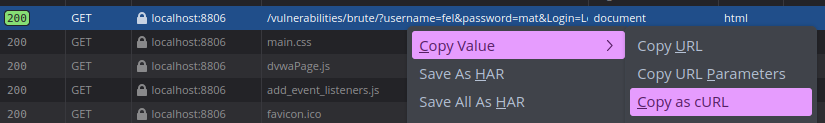
\includegraphics[width=0.85\textwidth]{img/07-1-obtencionCURLErroneo.png}
    \caption{Obtención del código cURL para un request GET con credenciales inválidas.}
    \label{fig:curlErroneo}
\end{figure}

A continuación, se realizó un inicio de sesión con credenciales válidas y se copió
el código cURL del request exitoso (Figura~\ref{fig:curlValido}).

\begin{figure}[H]
    \centering
    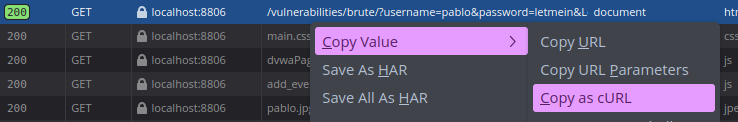
\includegraphics[width=0.85\textwidth]{img/07-2-obtencionCURLValido.png}
    \caption{Obtención del código cURL para un request GET con credenciales válidas.}
    \label{fig:curlValido}
\end{figure}

\subsection{Utilización de curl por terminal (curl)}

Los comandos cURL obtenidos desde las \textit{DevTools} del navegador fueron ejecutados
directamente en la terminal. En ambos casos se empleó el flag \texttt{-i}
(\textit{include}), el cual instruye a cURL para que incluya los encabezados de la
respuesta HTTP en la salida estándar, precediendo al cuerpo HTML. Esto permite
inspeccionar el código de estado, el tipo de contenido y otros metadatos de la respuesta
sin necesidad de herramientas adicionales.

En primer lugar, se ejecutó el comando correspondiente al acceso con credenciales
inválidas. La respuesta del servidor retornó el código de estado \texttt{200 OK}
(Figura~\ref{fig:curlInvalido}).

\begin{figure}[H]
    \centering
    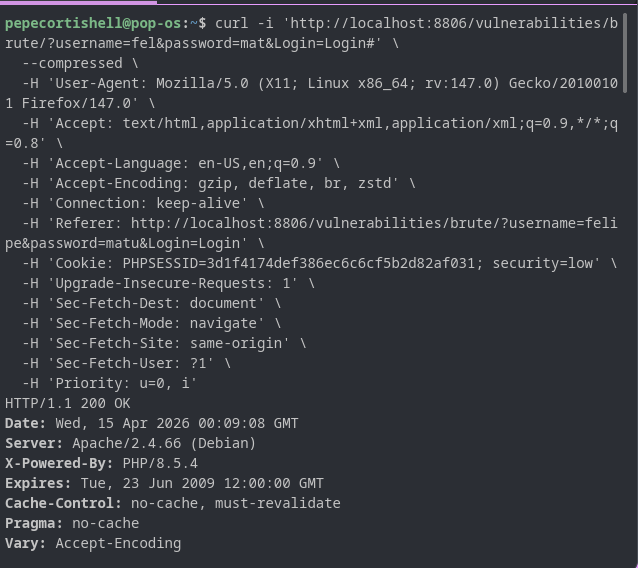
\includegraphics[width=0.85\textwidth]{img/08-1-curlInvalido.png}
    \caption{Ejecución del comando cURL con credenciales inválidas. Se aprecian los encabezados de respuesta HTTP seguidos del cuerpo HTML.}
    \label{fig:curlInvalido}
\end{figure}

A continuación, se ejecutó el comando con credenciales válidas
(\texttt{pablo / letmein}). La respuesta del servidor retornó igualmente
el código de estado \texttt{200 OK} (Figura~\ref{fig:curlValido}).

\begin{figure}[H]
    \centering
    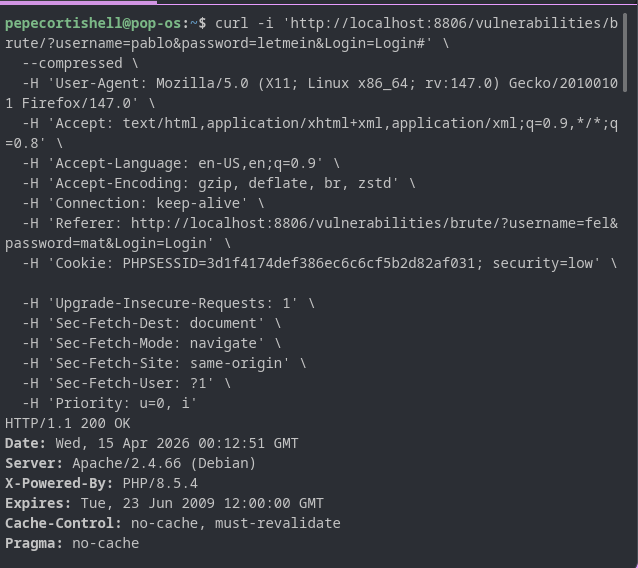
\includegraphics[width=0.85\textwidth]{img/08-2-curlValido.png}
    \caption{Ejecución del comando cURL con credenciales válidas. El cuerpo de la respuesta contiene el mensaje de bienvenida.}
    \label{fig:curlValido}
\end{figure}

\subsection{Demuestra 4 diferencias (curl)}

En la Tabla~\ref{tab:diferencias} se presentan las 4 diferencias identificadas entre
las respuestas HTTP obtenidas ante un acceso válido e inválido al formulario de
\texttt{/vulnerabilities/brute/}.

\begin{table}[H]
    \centering
    \caption{Diferencias entre la respuesta HTTP ante acceso válido e inválido.}
    \label{tab:diferencias}
    \small
    \begin{tabular}{P{3.4cm}P{4.2cm}P{4.5cm}}
        \toprule
        \textbf{Ubicación} & \textbf{Acceso inválido} & \textbf{Acceso válido} \\
        \midrule
        Header \texttt{Content-Length} & \texttt{1504} & \texttt{1527} \\
        \addlinespace
        Cuerpo HTML: mensaje de resultado & \textit{Username and/or password incorrect.} & \textit{Welcome to the password protected area pablo} \\
        \addlinespace
        Etiqueta HTML del mensaje & \texttt{<pre>} & \texttt{<p>} \\
        \addlinespace
        Imagen de usuario & No presente & \texttt{<img}\newline\texttt{src="/hackable/}\newline\texttt{users/pablo.jpg">} \\
        \bottomrule
    \end{tabular}
\end{table}

\subsection{Instalaci\'{o}n y versi\'{o}n a utilizar (hydra)}

Se instaló Hydra en el equipo mediante el gestor de paquetes del sistema operativo,
ejecutando el comando \texttt{sudo apt install hydra}
(Figura~\ref{fig:installHydra}).

\begin{figure}[H]
    \centering
    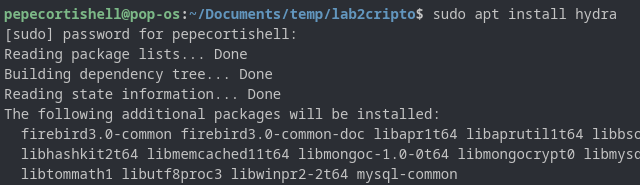
\includegraphics[width=0.85\textwidth]{img/10-1-installHydra.png}
    \caption{Instalación de Hydra mediante \texttt{apt}.}
    \label{fig:installHydra}
\end{figure}

La correcta instalación y la versión disponible se verificaron ejecutando
\texttt{hydra -h}, que despliega la ayuda de la herramienta junto con el número de
versión (Figura~\ref{fig:hydraVersion}).

\begin{figure}[H]
    \centering
    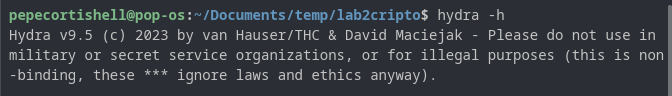
\includegraphics[width=0.85\textwidth]{img/10-2-hydraversion.png}
    \caption{Verificación de la versión instalada de Hydra mediante \texttt{hydra -h}.}
    \label{fig:hydraVersion}
\end{figure}

\subsection{Explicación de comando a utilizar (hydra)}

Para realizar el ataque de fuerza bruta con Hydra, se configuró la herramienta para iterar sobre un diccionario de usuarios y un diccionario de contraseñas, reemplazando dinámicamente estos valores en los parámetros de la petición HTTP. Se estableció como criterio de éxito la presencia de la palabra \textit{Welcome} en la respuesta del servidor, lo que permite identificar las credenciales válidas. Finalmente, los pares correctos obtenidos durante el ataque se almacenan en un archivo de resultados.

La Tabla~\ref{tab:hydraParams} describe cada parámetro empleado en la ejecución.

\begin{table}[H]
    \centering
    \caption{Parámetros del comando Hydra utilizado en el ataque.}
    \label{tab:hydraParams}
    \small
    \begin{tabular}{P{3.5cm}P{8cm}}
        \toprule
        \textbf{Parámetro} & \textbf{Descripción} \\
        \midrule
        \texttt{-L u.txt}         & Lista de usuarios a probar. \\
        \addlinespace
        \texttt{-P p.txt}         & Lista de contraseñas a probar. \\
        \addlinespace
        \texttt{localhost -s 8806} & Servidor objetivo y puerto. \\
        \addlinespace
        \texttt{http-get-form}    & Módulo de Hydra para formularios HTTP con método GET. \\
        \addlinespace
        Cadena de formulario & Configuración del endpoint para el módulo \texttt{http-get-form}, compuesta por tres campos separados por \texttt{:}: (1) ruta del endpoint, (2) parámetros con marcadores \texttt{\^{}USER\^{}} y \texttt{\^{}PASS\^{}} que Hydra reemplaza en cada intento, (3) cabecera \texttt{Cookie} con \texttt{PHPSESSID} y condición de éxito \texttt{S=Welcome}. \\
        \addlinespace
        \texttt{-o resultados.txt} & Archivo de salida donde se guardan las credenciales válidas encontradas. \\
        \addlinespace
        \texttt{-vV}              & Modo verbose: muestra en pantalla cada intento realizado. \\
        \bottomrule
    \end{tabular}
\end{table}

\begin{figure}[H]
    \centering
    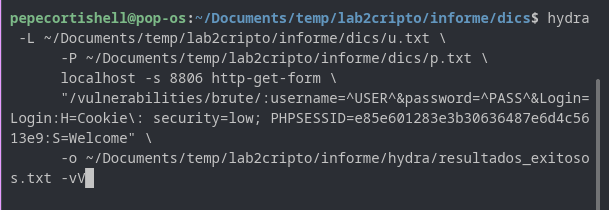
\includegraphics[width=0.85\textwidth]{img/11-1-hydraScript.png}
    \caption{Script bash con el comando Hydra configurado para el ataque de fuerza bruta.}
    \label{fig:hydraScript}
\end{figure}

\subsection{Obtenci\'{o}n de al menos 2 pares (hydra)}

Durante la ejecución de la herramienta, se mostraron en la consola los intentos realizados y los resultados obtenidos en tiempo real, gracias al uso del parámetro \texttt{-vV}. Como se puede observar en la Figura~\ref{fig:resultadosHydra}, se logró identificar exitosamente dos pares de credenciales válidas: el usuario \texttt{1337} con la contraseña \texttt{charley}, y el usuario \texttt{smithy} con la contraseña \texttt{password}.

\begin{figure}[H]
    \centering
    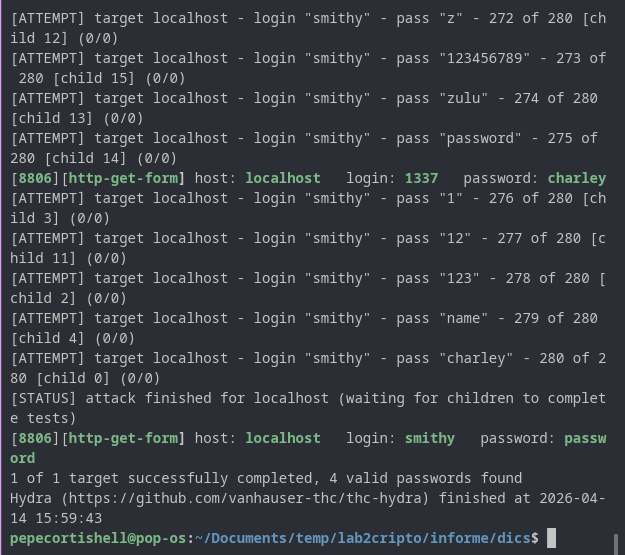
\includegraphics[width=0.85\textwidth]{img/12-1-resultadosScript.png}
    \caption{Ejecución del ataque con Hydra donde se identifican credenciales válidas.}
    \label{fig:resultadosHydra}
\end{figure}

\subsection{Explicación paquete curl (tráfico)}

\subsection{Explicación paquete burp (tráfico)}

\subsection{Explicación paquete hydra (tráfico)}

\subsection{Mención de las diferencias (tráfico)}

\subsection{Detección de SW (tráfico)}

\subsection{Interacción con el formulario (python)}

Para automatizar la interacción con el formulario ubicado en \texttt{vulnerabilities/brute/}, se elaboró un script en Python. En su configuración inicial, el código requiere la definición de variables internas clave: la URL del objetivo, las rutas hacia los archivos de diccionario de usuarios y contraseñas, y un identificador de sesión (\texttt{PHPSESSID}) válido obtenido tras una autenticación manual previa (Figura~\ref{fig:pythonVars}).

\begin{figure}[H]
    \centering
    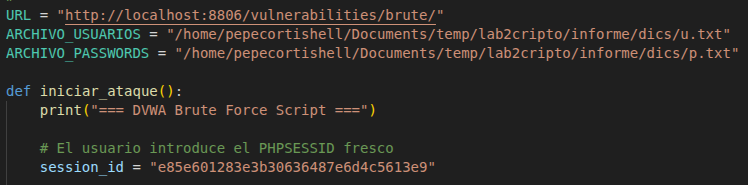
\includegraphics[width=0.85\textwidth]{img/18-1-URLySESSION.png}
    \caption{Configuración de la URL, diccionarios y \texttt{session\_id} en el script de Python.}
    \label{fig:pythonVars}
\end{figure}

El núcleo del funcionamiento del script radica en un proceso iterativo que recorre todas las combinaciones posibles entre los usuarios y las contraseñas provistas por los diccionarios. En cada ciclo, ambos valores son inyectados como parámetros dentro de una solicitud HTTP \texttt{GET}. Dicha solicitud es enviada junto a las \textit{cookies} correspondientes y las cabeceras (\textit{headers}) necesarias para simular la petición legítima de un navegador, permitiendo así que la aplicación evalúe el inicio de sesión (Figura~\ref{fig:pythonIteracion}).

\begin{figure}[H]
    \centering
    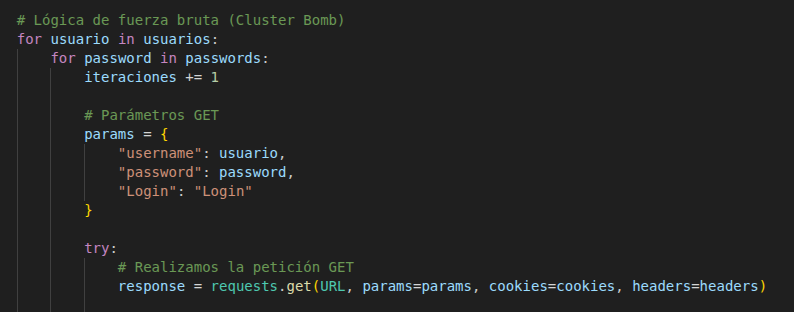
\includegraphics[width=0.85\textwidth]{img/18-2-iteracionCodigo.png}
    \caption{Lógica de iteración y construcción de la petición \texttt{GET} en el código Python.}
    \label{fig:pythonIteracion}
\end{figure}

\subsection{Cabeceras HTTP (python)}

Para la correcta ejecución del script, las peticiones requerían la inclusión de cabeceras HTTP (\textit{headers}). Estas fueron definidas de manera manual dentro del código; específicamente, el \texttt{User-Agent} se configuró con un valor arbitrario y personalizado, mientras que las demás características fueron copiadas textualmente a partir de las cabeceras generadas implícitamente durante las pruebas iniciales con cURL (Figura~\ref{fig:pythonHeaders}).

\begin{figure}[H]
    \centering
    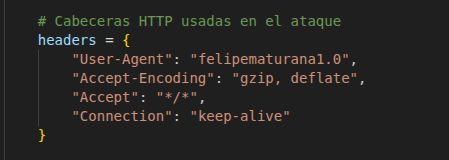
\includegraphics[width=0.85\textwidth]{img/19-1-headers.png}
    \caption{Definición de las cabeceras HTTP utilizadas en el script de Python.}
    \label{fig:pythonHeaders}
\end{figure}

En la Tabla~\ref{tab:pythonHeaders} se describe brevemente la funcionalidad de cada uno de los parámetros que fueron incorporados en la configuración de la petición.

\begin{table}[H]
    \centering
    \caption{Cabeceras HTTP definidas en el script y su propósito.}
    \label{tab:pythonHeaders}
    \small
    \begin{tabular}{P{3.5cm}P{8cm}}
        \toprule
        \textbf{Cabecera} & \textbf{Descripción} \\
        \midrule
        \texttt{User-Agent}      & Identifica al cliente (navegador o aplicación) que realiza la petición. Se definió con el valor arbitrario \texttt{felipematurana1.0} para simular una aplicación particular. \\
        \addlinespace
        \texttt{Accept-Encoding} & Informa al servidor sobre los algoritmos de compresión que el cliente soporta, como \texttt{gzip, deflate}, optimizando el ancho de banda. \\
        \addlinespace
        \texttt{Accept}          & Determina el formato de contenido que el cliente espera y puede procesar. El valor \texttt{*/*} indica que se acepta cualquier tipo de respuesta. \\
        \addlinespace
        \texttt{Connection}      & Especifica si la conexión de red debe permanecer abierta (\texttt{keep-alive}) para futuras peticiones, lo que es ideal para ataques iterativos. \\
        \bottomrule
    \end{tabular}
\end{table}

\subsection{Obtención de al menos 2 pares (python)}

Una vez finalizada la ejecución del script de Python, este genera de manera automática un archivo de resultados a modo de reporte. Este documento condensa los datos del ataque, mostrando el tiempo total que demoró el proceso completo y la cantidad exacta de iteraciones realizadas. Adicionalmente, el archivo lista las cabeceras HTTP empleadas durante las peticiones y expone los pares válidos de usuario y contraseña que lograron una autenticación exitosa (Figura~\ref{fig:pythonResultados}).

\begin{figure}[H]
    \centering
    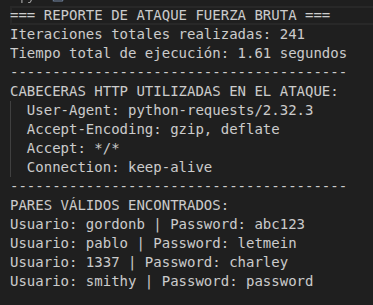
\includegraphics[width=0.85\textwidth]{img/20-1-resultadosPython.png}
    \caption{Archivo de resultados generado por el script en Python exhibiendo los pares válidos hallados.}
    \label{fig:pythonResultados}
\end{figure}

\subsection{Comparación de rendimiento con Hydra, Burpsuite, y cURL (python)}

Con el propósito de comparar el rendimiento de las distintas herramientas empleadas, se elaboró un script en bash que registra el tiempo de inicio y de término de la ejecución del ataque de fuerza bruta tanto para cURL como para Hydra. El script en Python ya incorporaba internamente esta medición de manera nativa. En el caso de Burp Suite Community Edition, la herramienta aplica un límite de velocidad que introduce un retardo fijo por cada petición enviada, retardo que además crece de forma proporcional a la cantidad de peticiones realizadas; dado que este valor no es constante ni configurable en su versión gratuita, se asumió un valor arbitrario de 0,5 segundos por petición, lo que, para un total de 280 combinaciones, resulta en un tiempo estimado de 140 segundos.

Para obtener valores representativos, cada herramienta fue ejecutada en múltiples oportunidades y se calculó el promedio de los tiempos registrados. Los resultados obtenidos se resumen en la Tabla~\ref{tab:rendimiento}.

\begin{table}[H]
    \centering
    \caption{Comparación del tiempo promedio de ejecución del ataque de fuerza bruta (280 combinaciones) por herramienta.}
    \label{tab:rendimiento}
    \small
    \begin{tabular}{P{3.5cm}P{2.5cm}P{2.5cm}P{2.5cm}P{2.5cm}}
        \toprule
        \textbf{Métrica} & \textbf{Burp Suite} & \textbf{cURL} & \textbf{Hydra} & \textbf{Python} \\
        \midrule
        Tiempo promedio (280 combinaciones) & $\approx$ 140,00 s & 5,70 s & 4,37 s & 1,74 s \\
        \bottomrule
    \end{tabular}
\end{table}


\newpage
\subsection{Demuestra 4 métodos de mitigación (investigación)}

% Please add the following required packages to your document preamble:
%\begin{table}[htbp]

\section*{Conclusiones y comentarios}

\end{document}
